% Requires: amsmath, booktabs, graphicx, siunitx (v3: \qty, \unit)
% Figure asset: plot_iteration_knee.png  (generated by plot_iteration_knee.py)
% Data: synth_job_batches/iteration_sweep_summary-21.csv
\section{Iteration Scaling and the Onset of Quantum Congestion}
\label{sec:iteration-scaling}

Variational algorithms are defined by their outer loop: a VQE or QAOA instance
is not one circuit but $k$ rounds of circuit execution followed by classical
parameter update. Cost models for hybrid clouds almost universally treat this
loop as a multiplier --- $k$ iterations cost $k$ times one iteration. This
section shows that the multiplier assumption fails, and fails abruptly. Beyond
a critical iteration count the marginal cost of one additional iteration rises
by more than an order of magnitude, while the classical half of the very same
workload continues to scale perfectly linearly. The effect is invisible to any
model that does not represent device occupancy, because it is not a property of
the workload at all: it is a property of the interaction between the workload
and a finite quantum fleet.

\subsection{Experimental Design}
\label{sec:iter-setup}

The experiment is a single-factor sweep. We generate one batch of
$N=3000$ synthetic variational jobs and replicate it seven times, altering
exactly one field --- the requested iteration count
$k \in \{3,6,9,12,15,18,21\}$. Every other job attribute is bit-identical
across the seven traces: qubit width, circuit depth, shot count, priority,
arrival timestamp, CPU core demand, and memory bandwidth demand. Any difference
in the measured outcome is therefore attributable to $k$ alone, with no
confounding from workload composition or arrival pattern.

Jobs request $10$--$20$ qubits (mean $15.15$), circuit depth $10$--$20$,
$2000$--$9000$ shots (mean $5501$), $7$--$10$ CPU units, and $14$--$20$
memory-bandwidth units. Arrivals are replayed from the trace over a window of
$2884.8$ time units, giving a mean arrival rate
$\lambda = 1.04$ jobs per unit time.

The target platform is a fixed hybrid inventory: two superconducting QPUs
modeled on IBM Eagle~r3 devices (\texttt{IBM\_Strasbourg} as QPU-1 and
\texttt{IBM\_Brussels} as QPU-2, $127$ physical qubits each, with their
published CLOPS, quantum volume, and $T_1/T_2$ figures), and two
\texttt{AMDRyzen} classical nodes. Devices are instantiated afresh for every
run so that no qubit-occupancy or topology state leaks between configurations.
Energy is attributed with a constant cryogenic draw of $\qty{70}{\kilo\watt}$
for QPU-1 and $\qty{60}{\kilo\watt}$ for QPU-2, an affine CPU power model, and
an electricity price of $\$0.18$ per \unit{\kilo\watt\hour}. Each of the seven
configurations is executed to completion and summarized over all $3000$ jobs.

Two structural features of the platform matter for what follows. First, a QPU
admits several jobs concurrently, bounded not by a job slot count but by free
qubits: at a mean width of $15.15$ qubits, the $254$-qubit fleet could in
principle host $C \approx 16.8$ jobs at once. Second, admission is resolved at
two levels --- aggregate qubit capacity \emph{and} physical connectivity. A job
is admitted only when a \emph{connected} subgraph of free qubits exists, so the
achievable concurrency is strictly below $C$ whenever the free qubits are
scattered across the coupling graph.

It is convenient to summarize the offered load by the dimensionless ratio
\begin{equation}
  \rho(k) \;=\; \frac{\lambda \, s_1 \, k}{C},
  \label{eq:rho}
\end{equation}
where $s_1 = \qty{0.97}{\second}$ is the uncontended QPU service time of a
single iteration, measured at the smallest sweep point. Equation~\eqref{eq:rho}
is the fraction of nominal fleet concurrency that the workload demands; it rises
from $\rho = 0.18$ at $k=3$ to $\rho = 1.27$ at $k=21$.

\subsection{Metrics and Figure Construction}
\label{sec:iter-metrics}

Plotting a quantity that grows by two orders of magnitude against a variable
that grows by one produces a curve that is steep everywhere and informative
nowhere. Figure~\ref{fig:iteration-knee} therefore reports three
\emph{derived}, scale-free views of the same sweep, each chosen so that the
linear-scaling null hypothesis appears as a flat line. Departure from linearity
is then visible as departure from flatness, rather than having to be inferred
from the curvature of a monotone climb.

\paragraph{Panel (a): marginal cost of one iteration.}
We divide the mean per-job QPU and CPU phase times by $k$, giving the average
cost of a single iteration on each resource class. Under the multiplier
assumption both series are horizontal. Because the two series share a unit
(\unit{\second} per iteration) they share one axis; the axis is logarithmic
because the QPU series spans a factor of $41$ while the CPU series does not
move. We label the ordinate ``service $+$ blocking'' deliberately --- see
Section~\ref{sec:iter-validity}.

\paragraph{Panel (b): local scaling exponent.}
For consecutive sweep points we estimate the finite-difference log--log slope
of per-job total energy,
\begin{equation}
  \alpha(k) \;=\;
  \frac{\ln E_{i+1} - \ln E_{i}}{\ln k_{i+1} - \ln k_{i}},
  \label{eq:alpha}
\end{equation}
and plot it at the geometric midpoint $\sqrt{k_i k_{i+1}}$ of each bracket.
This is the instantaneous exponent of the relation $E \propto k^{\alpha}$:
$\alpha = 1$ is exactly the multiplier assumption and is drawn as a reference
line. The estimator localizes the departure from linearity to a bracket, which
a global power-law fit --- which would report a single misleading average
exponent over a two-regime curve --- cannot do.

\paragraph{Panel (c): dispersion and tail weight.}
We plot two dimensionless descriptors of the per-job turnaround distribution
\emph{within} each run: the coefficient of variation
$\mathrm{CV} = \sigma/\mu$, and the tail ratio $p_{95}/\mathrm{median}$. Both
are invariant to the overall time scale, so they isolate changes in the
\emph{shape} of the distribution from changes in its magnitude. The reference
line at $\mathrm{CV}=1$ marks exponential-like dispersion, the canonical
signature of a queue that has begun to build.

In all three panels a shaded band marks the congested regime, with its left
edge at the midpoint of the $k=9 \rightarrow 12$ bracket in which the exponent
of Eq.~\eqref{eq:alpha} first leaves unity. The figure is generated from the
sweep summary by \texttt{plot\_iteration\_knee.py}; no smoothing, fitting, or
interpolation is applied, and every plotted value is a direct arithmetic
transform of the tabulated measurements.

\begin{figure*}[t]
  \centering
  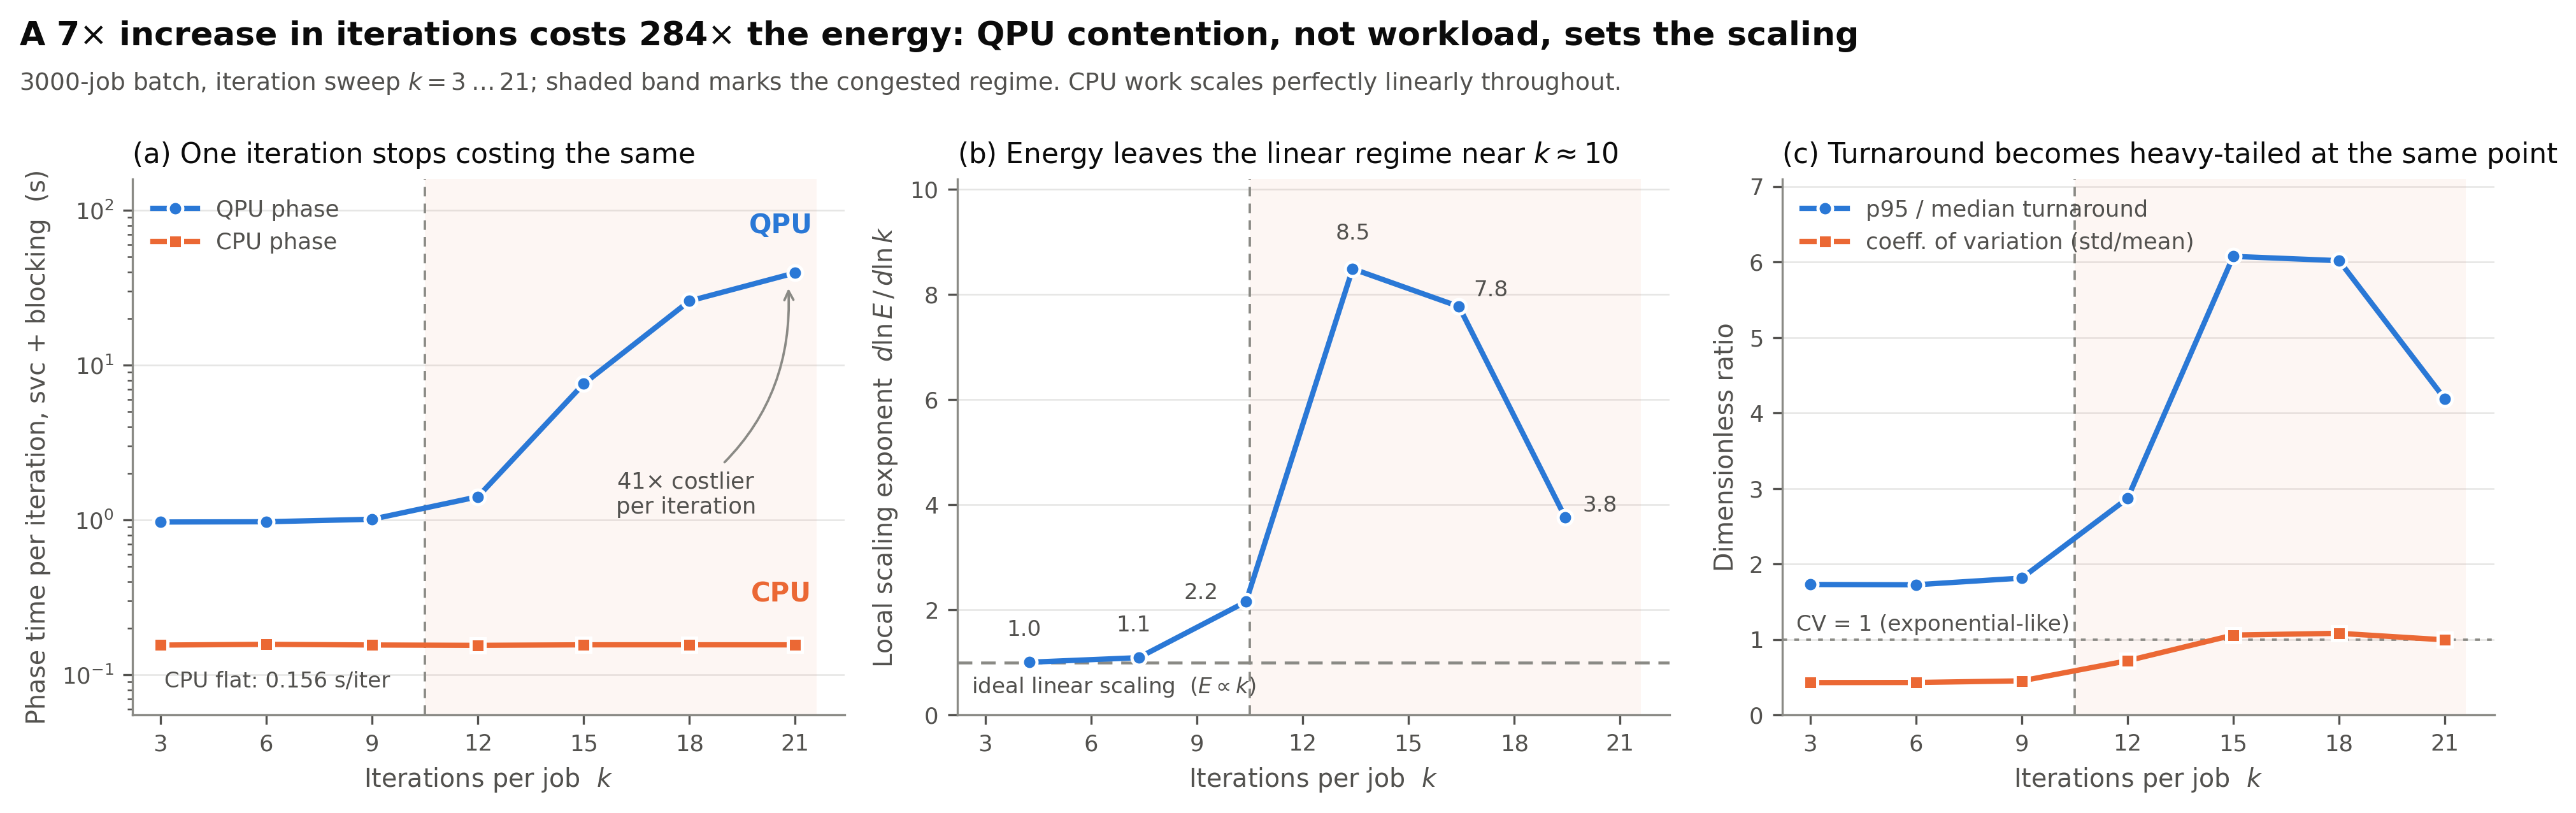
\includegraphics[width=\textwidth]{plot_iteration_knee.png}
  \caption{Iteration scaling of a fixed $3000$-job variational workload on a
    two-QPU, two-CPU hybrid fleet. Only the requested iteration count $k$
    varies across the seven runs. (a)~Phase time normalized per iteration: the
    classical phase is flat at \qty{0.156}{\second} per iteration to within
    $1\%$ across the entire sweep, while the quantum phase becomes $41\times$
    more expensive per iteration. (b)~Local scaling exponent
    $\alpha = \mathrm{d}\ln E / \mathrm{d}\ln k$ of per-job energy against the
    ideal-linear reference $\alpha=1$. (c)~Turnaround dispersion: the
    coefficient of variation crosses unity, and the $p_{95}$/median ratio more
    than triples, in the same bracket in which $\alpha$ departs from~$1$.}
  \label{fig:iteration-knee}
\end{figure*}

\begin{table}[t]
\centering
\caption{Iteration sweep over an identical $3000$-job trace. $\rho$ is the
offered concurrency of Eq.~\eqref{eq:rho}; per-iteration columns are mean phase
time divided by $k$; $E$ is mean per-job total energy.}
\label{tab:iteration-sweep}
\small
\setlength{\tabcolsep}{4.5pt}
\begin{tabular}{@{}rrrrrrr@{}}
\toprule
 & & \multicolumn{2}{c}{Per iteration (\unit{\second})}
 & & \multicolumn{2}{c}{Turnaround} \\
\cmidrule(lr){3-4}\cmidrule(lr){6-7}
$k$ & $\rho$ & QPU & CPU & $E$ (\unit{\kilo\watt\hour})
 & CV & $p_{95}/\tilde{x}$ \\
\midrule
 3 & 0.18 &  0.97 & 0.156 &  0.053 & 0.43 & 1.73 \\
 6 & 0.36 &  0.97 & 0.157 &  0.107 & 0.43 & 1.72 \\
 9 & 0.54 &  1.01 & 0.156 &  0.167 & 0.45 & 1.81 \\
\midrule
12 & 0.72 &  1.41 & 0.155 &  0.310 & 0.72 & 2.87 \\
15 & 0.90 &  7.58 & 0.156 &  2.057 & 1.06 & 6.07 \\
18 & 1.08 & 25.99 & 0.156 &  8.484 & 1.08 & 6.02 \\
21 & 1.27 & 39.50 & 0.156 & 15.159 & 0.99 & 4.19 \\
\bottomrule
\end{tabular}
\end{table}

\subsection{Results}
\label{sec:iter-results}

\paragraph{The classical half of the workload is a control.}
The single most useful measurement in Table~\ref{tab:iteration-sweep} is the
CPU column, because it does not move. Per-iteration classical phase time is
\qty{0.156}{\second} at $k=3$ and \qty{0.156}{\second} at $k=21$, constant to
within $1\%$ across a sevenfold increase in loop length. The classical nodes
process exactly $7\times$ the work in $7\times$ the time. This is what
correct linear scaling looks like, measured on the same runs, under the same
scheduler, in the same simulator --- which forecloses the explanation that the
superlinearity reported below is an artifact of the harness. Whatever happens
at large $k$ happens to the quantum resource specifically.

\paragraph{The marginal iteration stops costing the same.}
Through $k=9$, the quantum phase also behaves as the multiplier assumption
predicts: $0.97$, $0.97$, and \qty{1.01}{\second} per iteration. Then it breaks.
The per-iteration cost rises to $1.41$ at $k=12$, $7.58$ at $k=15$, $25.99$ at
$k=18$, and \qty{39.50}{\second} at $k=21$ --- a $41\times$ inflation of the
marginal iteration. A job that asks for $21$ iterations does not receive $21$
copies of the iteration that a $k=3$ job receives; it receives $21$ iterations
that are each vastly more expensive, because by then the fleet it is running on
is congested by jobs exactly like itself.

\paragraph{Energy leaves the linear regime near $k \approx 10$.}
Panel~(b) localizes the transition. The exponent of Eq.~\eqref{eq:alpha} is
$1.00$ over the $3\rightarrow 6$ bracket and $1.09$ over $6 \rightarrow 9$ ---
statistically indistinguishable from the multiplier assumption. It reaches
$2.2$ over $9 \rightarrow 12$ and peaks at $8.5$ over $12 \rightarrow 15$. In
aggregate, raising $k$ from $3$ to $21$ --- a factor of~$7$ --- multiplies
per-job energy by~$284$ and per-job energy cost by the same factor, from
$\$0.0096$ to $\$2.73$. At fleet scale the identical $3000$-job workload
consumes \qty{160}{\kilo\watt\hour} at $k=3$ and
\qty{45477}{\kilo\watt\hour} at $k=21$: the same science, the same circuits,
the same arrival pattern, and a bill that moves from $\$29$ to $\$8186$.

\paragraph{Predictability collapses at the same point.}
Panel~(c) supplies an independent confirmation from a quantity the first two
panels never touch: the shape of the turnaround distribution. Through $k=9$
turnaround is tight and predictable, with $\mathrm{CV} \approx 0.44$ and a
$p_{95}$ only $1.8\times$ the median. In the $9 \rightarrow 12$ bracket --- the
same bracket in which $\alpha$ departs from unity --- the CV jumps to $0.72$
and then crosses~$1$, and the tail ratio more than triples to $6.07$. The
service-level consequence is concrete: in the linear regime an operator can
quote a $p_{95}$ completion time less than twice the median, and past the knee
cannot. Three quantities that are computed from different columns of the
measurement record --- marginal service time, energy exponent, and distribution
shape --- change character in the same interval. That coincidence is the
evidence that a single mechanism is responsible.

\paragraph{The mechanism is occupancy, not work.}
The offered-load column of Table~\ref{tab:iteration-sweep} identifies that
mechanism. Because a job's iterations are serialized --- each a QPU phase
followed by a CPU phase --- raising $k$ does not raise the work per iteration;
it raises how long the job \emph{resides} in the system. By Little's law the
mean population is $\lambda \bar{T}$, so a $k$-fold longer residency puts
$k$-fold more jobs on the fleet at once, each of them contending for qubits
during its quantum phases. Concurrency demand grows linearly in $k$, and the
knee falls at
$\rho \approx 0.5$--$0.7$: the fleet saturates while roughly a third of its
nominal qubit capacity is still formally free. The gap between saturation and
$\rho=1$ is the price of the connectivity constraint. Free qubits accumulate,
but scattered across the coupling graph, and a job requiring a connected
$15$-qubit region cannot use them. Beyond $k \geq 18$ the workload demands more
concurrency than the fleet nominally possesses ($\rho > 1$) and the system is
in overload, where turnaround is governed by backlog drain rather than by
service.

The energy consequence follows directly from the power model. A superconducting
QPU draws its full cryogenic baseline whenever it hosts a job, so energy is
charged for \emph{occupancy}, not for useful computation. Iterations spent
resident on a congested device --- including time spent holding qubits while
waiting for a connected region to open --- are billed at
\qty{70}{\kilo\watt}. This is why the energy exponent in panel~(b) tracks the
service-time inflation in panel~(a) so closely: they are, physically, the same
measurement. The share of per-job energy attributable to the QPU rises from
$98.4\%$ to $99.97\%$ over the sweep, so classical post-processing --- the part
of the pipeline that scales perfectly --- is also the part that never mattered
to the energy budget.

\subsection{Implications}
\label{sec:iter-implications}

The practical reading is that iteration count is not a workload parameter to be
optimized in isolation by the algorithm designer; it is a
\emph{capacity-planning} parameter with a threshold. An operator sizing a fleet
from single-job measurements at small $k$ will extrapolate linearly and
under-provision by two orders of magnitude at $k=21$. A pricing scheme that
charges per iteration is, past the knee, charging a fixed price for a service
whose cost to the provider has grown $41$-fold --- and charging the same price
to a $k=3$ user who imposes almost none of that cost. Conversely, an algorithm
designer who trades a longer optimization loop for a shallower circuit may be
making a strictly worse system-level trade even when the per-circuit metrics
improve.

The result also argues for admission control on the outer loop specifically.
Because the transition is driven by residency rather than by arrival rate,
capping the number of concurrently \emph{resident} long-loop jobs --- rather
than the arrival rate, the queue length, or the qubit count --- is the control
that acts directly on the mechanism. Evaluating such a policy is precisely the
kind of question the simulator exists to answer, and we leave it to future
work.

\subsection{Threats to Validity}
\label{sec:iter-validity}

Three limitations qualify these results.

First, the dispersion statistics in panel~(c) are computed \emph{across the
$3000$ jobs within a single run}, not across replicate runs. They characterize
how unevenly a given configuration treats its own jobs --- which is the
service-level quantity of interest --- but they are not confidence intervals,
and the sweep does not repeat each configuration under independent random
seeds. Because job service times draw on the simulator's random state, which is
not seeded by default, replicate runs would be needed before attaching
uncertainty to any single tabulated value. The regime change is far too large
to be run-to-run noise; the precise location of the knee within the
$9 \rightarrow 12$ bracket is not resolved by seven points.

Second, in the current instrumentation the recorded per-phase waiting time is
identically zero, and end-to-end turnaround equals the sum of the reported
phase durations. Blocking is therefore \emph{folded into} the reported phase
time rather than accounted separately, which is why
Figure~\ref{fig:iteration-knee}(a) is labeled ``service $+$ blocking.'' This
does not affect any total --- turnaround, energy, and cost are all correct,
since a job blocked while holding qubits genuinely occupies and powers the
device --- but it means the present data cannot decompose the $41\times$
inflation into contention for qubits versus fragmentation of the coupling
graph. Separating the two requires instrumenting the admission retry loop, and
would sharpen the mechanism argument of Section~\ref{sec:iter-results} from
inference to measurement.

Third, the exponent estimates in the overloaded regime ($\rho > 1$, i.e.
$k \geq 18$) should be read qualitatively. Once offered concurrency exceeds
fleet capacity, turnaround is dominated by drain of a backlog accumulated over
a finite arrival window, so $\alpha$ becomes sensitive to the length of that
window; this is the reason the estimate falls from $8.5$ to $3.8$ at the right
of panel~(b) rather than continuing to climb. The robust claim is the departure
of $\alpha$ from unity and the bracket in which it occurs, not the peak value
it attains.
